\justifying
\NSFCBodyText

\subsubsection{研究目标}

\textbf{总体目标}：建立面向不完备文本描述的地理实体关系证据表示与跨模态匹配方法，形成可复现的分层评测协议，使遥感图文检索在关系敏感场景下的失效模式可识别、可缓解、可归因。

三个具体目标与后文研究内容一一对应：

\begin{enumerate}
    \item \itemtitlefont{目标一（表示）：}建立地理实体关系证据的三态表示与可复核标注规范，使"已支持、明确冲突、未知"三种状态在图像级描述条件下可判定。判据是关系词表与证据字段规范定稿，且人工核验子集的标注者间一致性达到 Cohen's $\kappa \geq 0.7$\textbf{【暂定】}。
    \item \itemtitlefont{目标二（学习）：}提出仅对可核验关系施加约束、对未知关系屏蔽监督的跨模态匹配方法。判据是在三臂对照中，本方法相对"未知作负例"处理在关系挑战集上取得统计显著改善，且标准 mR 无显著下降。
    \item \itemtitlefont{目标三（验证）：}建立可归因的分层评测协议。判据是同域比较、去重后的迁移测试与数据独立测试分别报告，且在等参数量、等训练预算对照下改进依然成立。
\end{enumerate}

图~\ref{fig:framework}给出三个目标对应的研究内容、交付物及错误归因回流关系。

% F4: F04_总体框架-v2.png
\begin{figure}[!htbp]
    \centering
    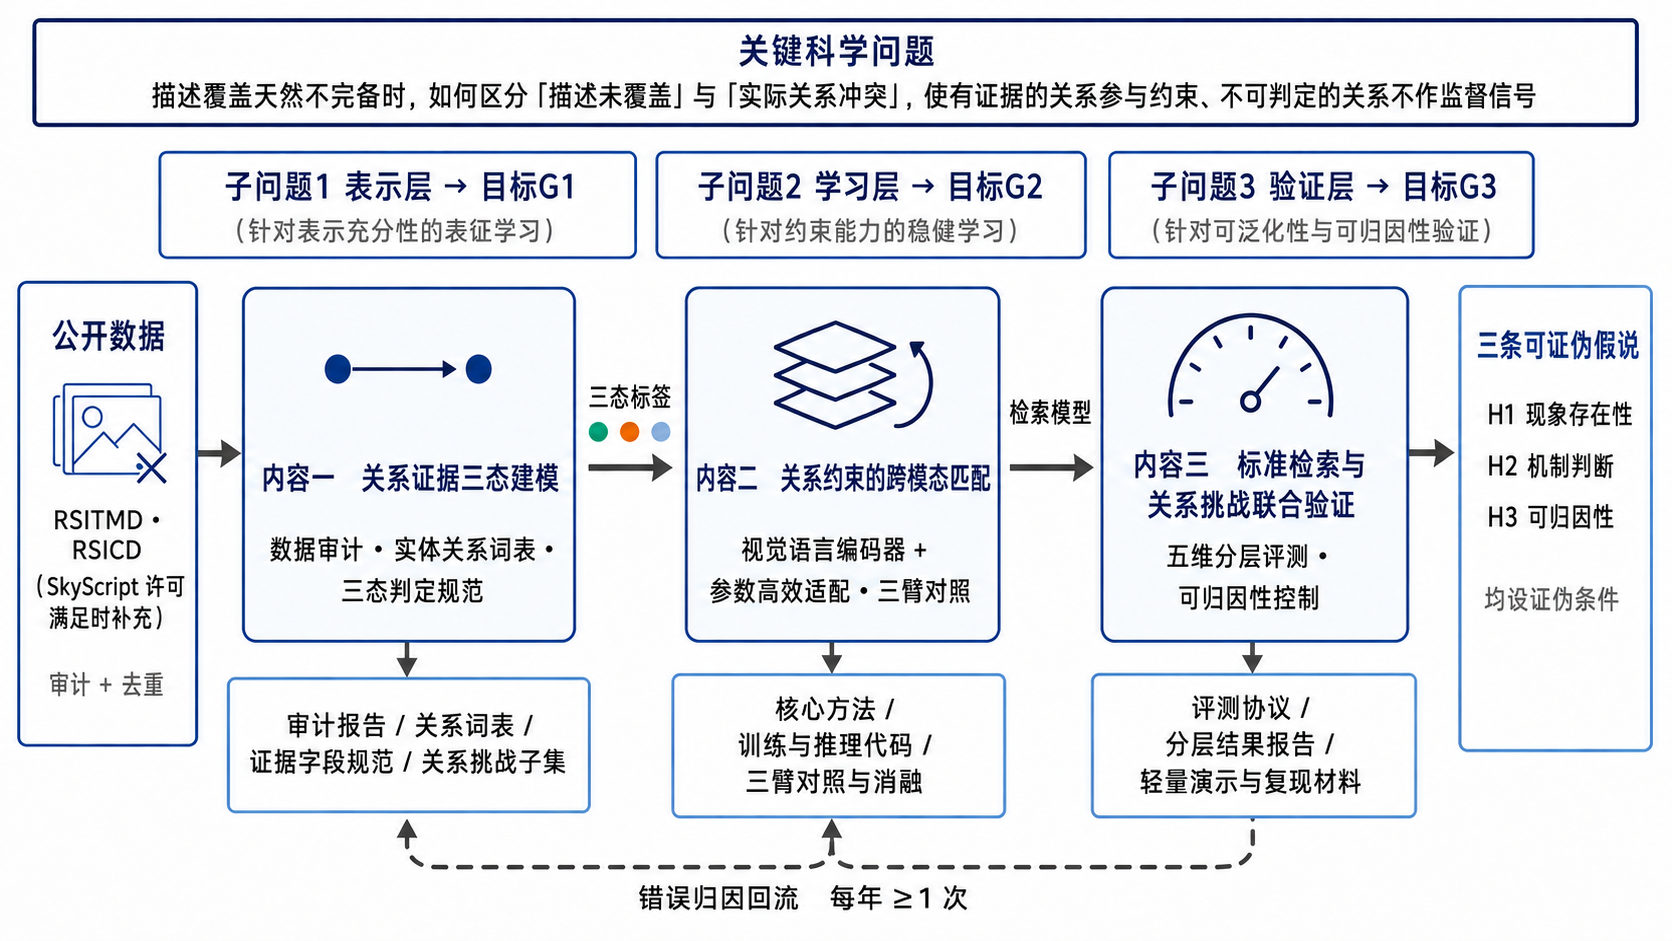
\includegraphics[width=\linewidth]{figures/F04_总体框架-v2.png}
    \caption{总体研究框架。三项内容依次支撑，并由联合验证的错误归因结果回流修订关系规范与匹配方法。}
    \label{fig:framework}
\end{figure}

\subsubsection{研究内容}

\subsubsubsection{内容一：不完备描述条件下的地理实体关系证据建模}

本内容回答"关系证据的三态如何可判、可复核地表示"。 具体技术路线见图~\ref{fig:route-one}。

% F5: F05_技术路线一-v2.png
\begin{figure}[!htbp]
    \centering
    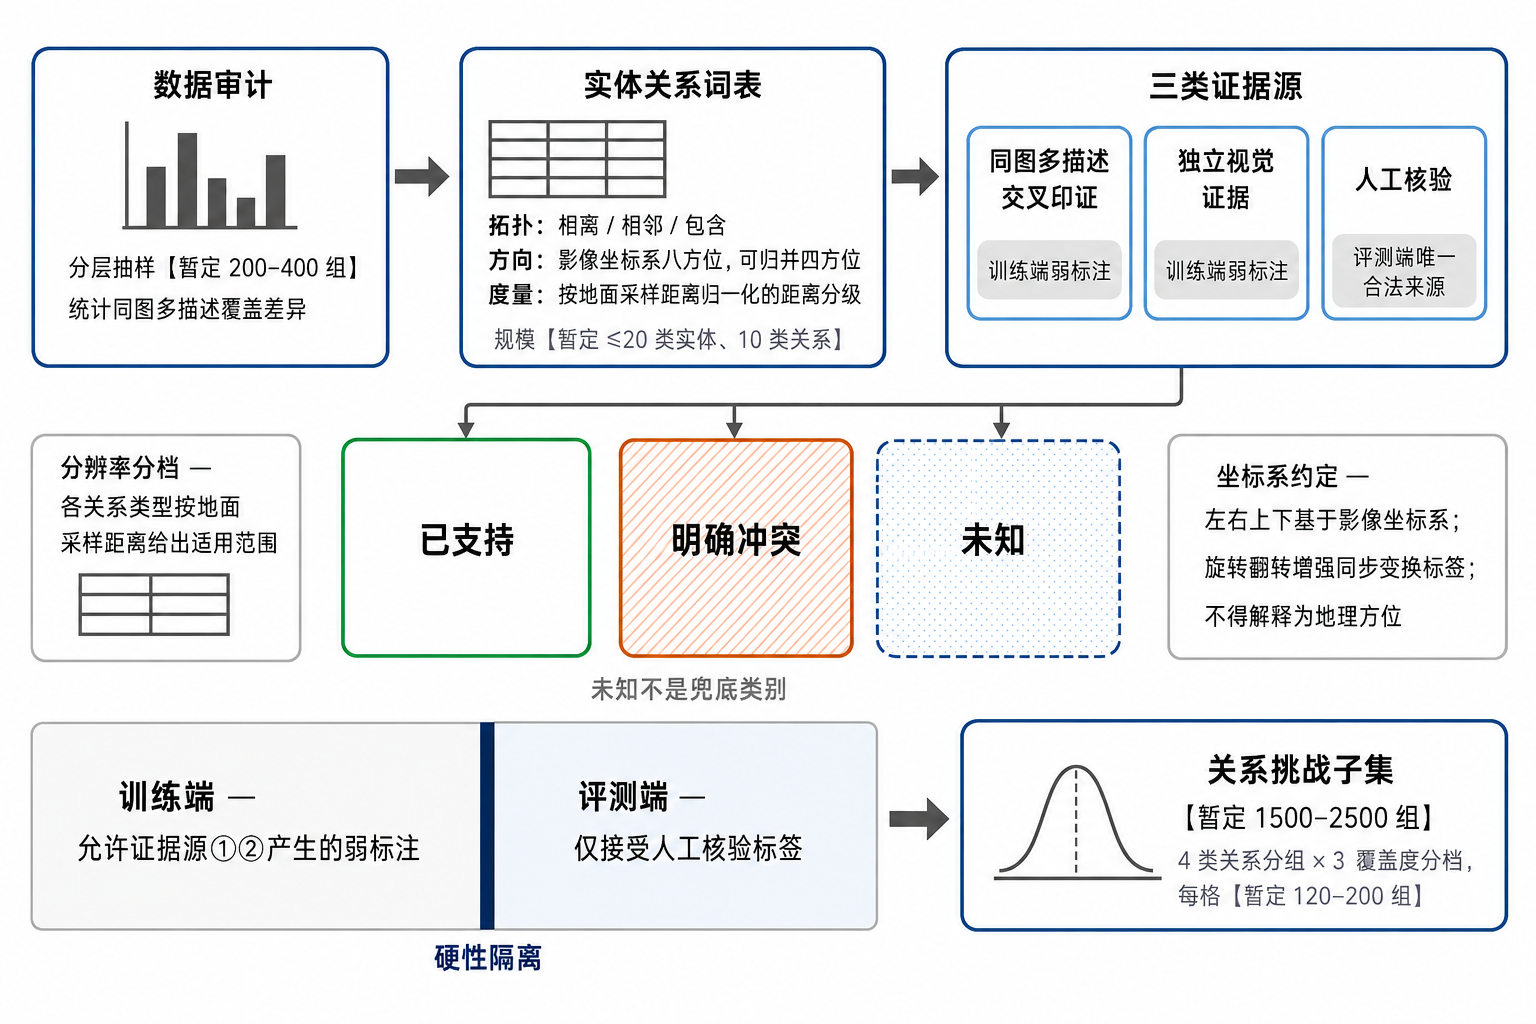
\includegraphics[width=\linewidth]{figures/F05_技术路线一-v2.png}
    \caption{技术路线一：关系证据三态建模。训练端弱标注与评测端人工核验严格分离，标注规模为暂定计划。}
    \label{fig:route-one}
\end{figure}


首先开展\textbf{公开数据审计}：对每个候选基准分层抽样\textbf{【暂定 200--400 组】}影像及其全部配对描述，逐组检查实体、关系、遗漏与矛盾，记录抽样规则与判定依据，统计同一影像多条描述之间的覆盖差异分布。这一步既是后续工作的数据基础，也是检验假说 H1 的直接证据来源。

其次\textbf{构建实体关系词表}：关系类型不从零定义，而是从地理信息科学已有的空间关系体系中取可判定的子集——拓扑关系取"相离、相邻、包含"三类，方向关系取基于影像坐标系的八方位并按需归并为四方位，度量关系取按地面采样距离归一化后的距离分级。实体类别由数据审计自下而上确定。整体规模控制在\textbf{【暂定 20 类实体、10 类关系】}以内，取舍依据是"该关系在给定分辨率的影像上能否被稳定判定"，而不是覆盖面。

再次\textbf{建立三态判定规范}，这是本内容的核心难点。在只有图像级描述、没有实体框与拓扑真值的条件下，判定"一条关系是否被影像支持"必须回答证据从何而来。本项目设定三类证据源，并规定其适用范围：

\begin{enumerate}
    \item \itemtitlefont{同图多描述的交叉印证（训练端弱标注）：}公开基准每幅影像配有 5 条独立撰写的描述\cite{lu2018rsicd,yuan2022amfmn}。若同一实体对的同一关系被两条及以上描述独立提及且互不矛盾，记为"已支持"候选；若不同描述对同一实体对给出互斥关系，记为"明确冲突"候选；仅被一条描述提及且无其它证据支持的，不升级为"已支持"。这一来源不引入任何外部模型，是最保守也最可靠的信号。
    \item \itemtitlefont{独立视觉证据（训练端弱标注）：}借助与被评测检索模型\textbf{不共享骨干与训练数据}的开放词汇检测或分割模型提供实体的位置与范围，再由\textbf{确定性几何规则}（外接框重叠、质心相对位置、归一化距离）计算拓扑、方向与度量关系。此处有一条必须坚持的约束：外部模型只负责\textbf{定位实体}，关系由几何规则判定，不由模型直接输出。这样做是为了避免用待检验的视觉语言模型去生成检验它自己的标签，从而陷入循环论证。
    \item \itemtitlefont{人工核验（评测端唯一合法来源）：}关系挑战子集的全部标签由标注人员直接对照影像判定，采用双人独立标注与第三人仲裁，并报告标注者间一致性。
\end{enumerate}

"未知"不是兜底类别，而是有判定条件的状态：实体无法被可靠定位、关系类型在该影像的地面采样距离下不可分辨、或各证据源相互矛盾且无法仲裁时，一律记为未知。分辨率是显式判据——同一关系在不同地面采样距离的影像上可判定性不同，判定规范按分辨率分档给出各关系类型的适用范围。

此外还有一条必须固定的技术约定：左右、上下等相对关系一律基于影像坐标系定义，训练中的旋转与翻转增强必须同步变换相应关系标签；影像内的相对位置不得直接解释为地理方位。 三类证据源、记录字段与未知态判据见图~\ref{fig:evidence-sources}。

% F8: F08_三类证据源与适用边界.png
\begin{figure}[!htb]
    \centering
    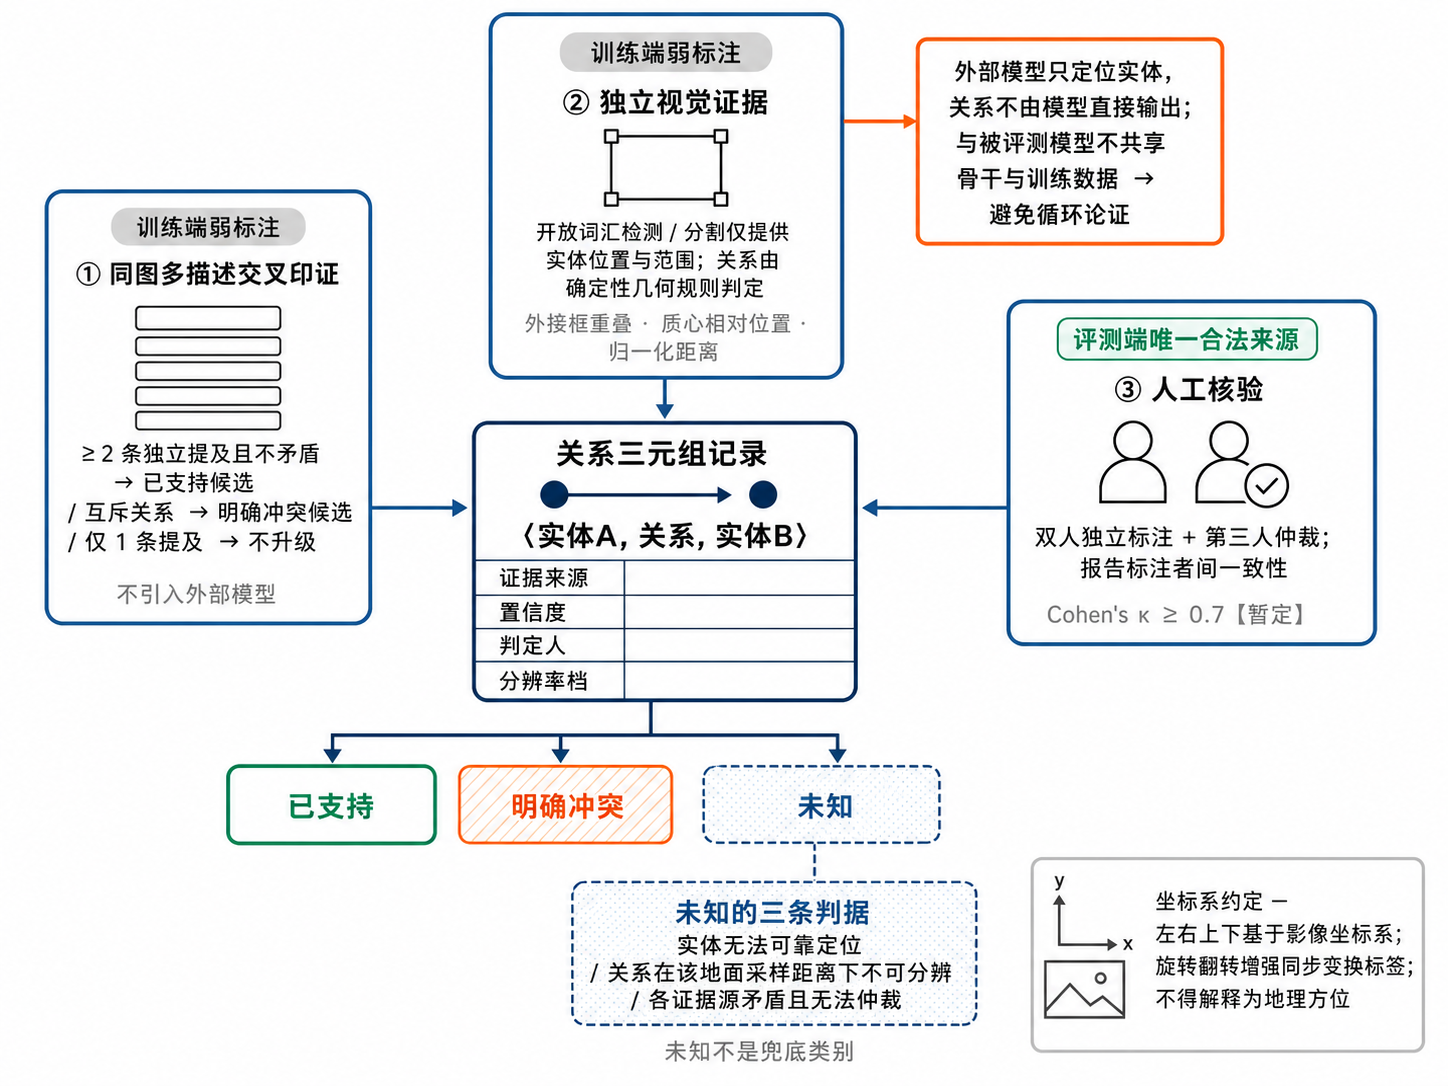
\includegraphics[width=\linewidth]{figures/F08_三类证据源与适用边界.png}
    \caption{三态判定的证据来源与适用边界。外部模型仅定位实体，关系由几何规则判定；评测标签全部经人工核验。}
    \label{fig:evidence-sources}
\end{figure}


最后\textbf{分离弱标注与人工核验}：训练集允许使用前两类证据源产生的弱标注，独立评测样本只接受人工核验标签。这一分离是本内容的底线——自动抽取结果属于弱监督，不能充当可信的测试标签。

关系挑战子集的规模按统计效力倒推确定，而不是先定数量再看能做什么。评测需要在"关系类型 × 覆盖度分档"上分层比较，若要在每个分层格内检出中等效应量、保持双侧显著性水平 0.05 与检验效能 0.8，每格约需 \textbf{【暂定 120--200 组】}样本；按 \textbf{【暂定 4 类关系分组 × 3 个覆盖度分档】}计算，总量约需 \textbf{【暂定 1500--2500 组】}。第一年完成审计后将依据实际效应量估计重新核定该规模；若分层过细导致每格样本不足，优先合并分档而非降低每格样本量。

本内容形成的交付物为：数据审计报告、实体关系词表、证据字段规范，以及经人工核验的关系挑战子集\textbf{【暂定 1500--2500 组】}。

\subsubsubsection{内容二：兼顾关系判别与未知信息的跨模态匹配}

本内容回答"三态信息以何种方式进入目标函数才有效"。 共享骨干下的三臂对照及候选实现方式见图~\ref{fig:route-two}。

% F6: F06_技术路线二-v2.png
\begin{figure}[!htbp]
    \centering
    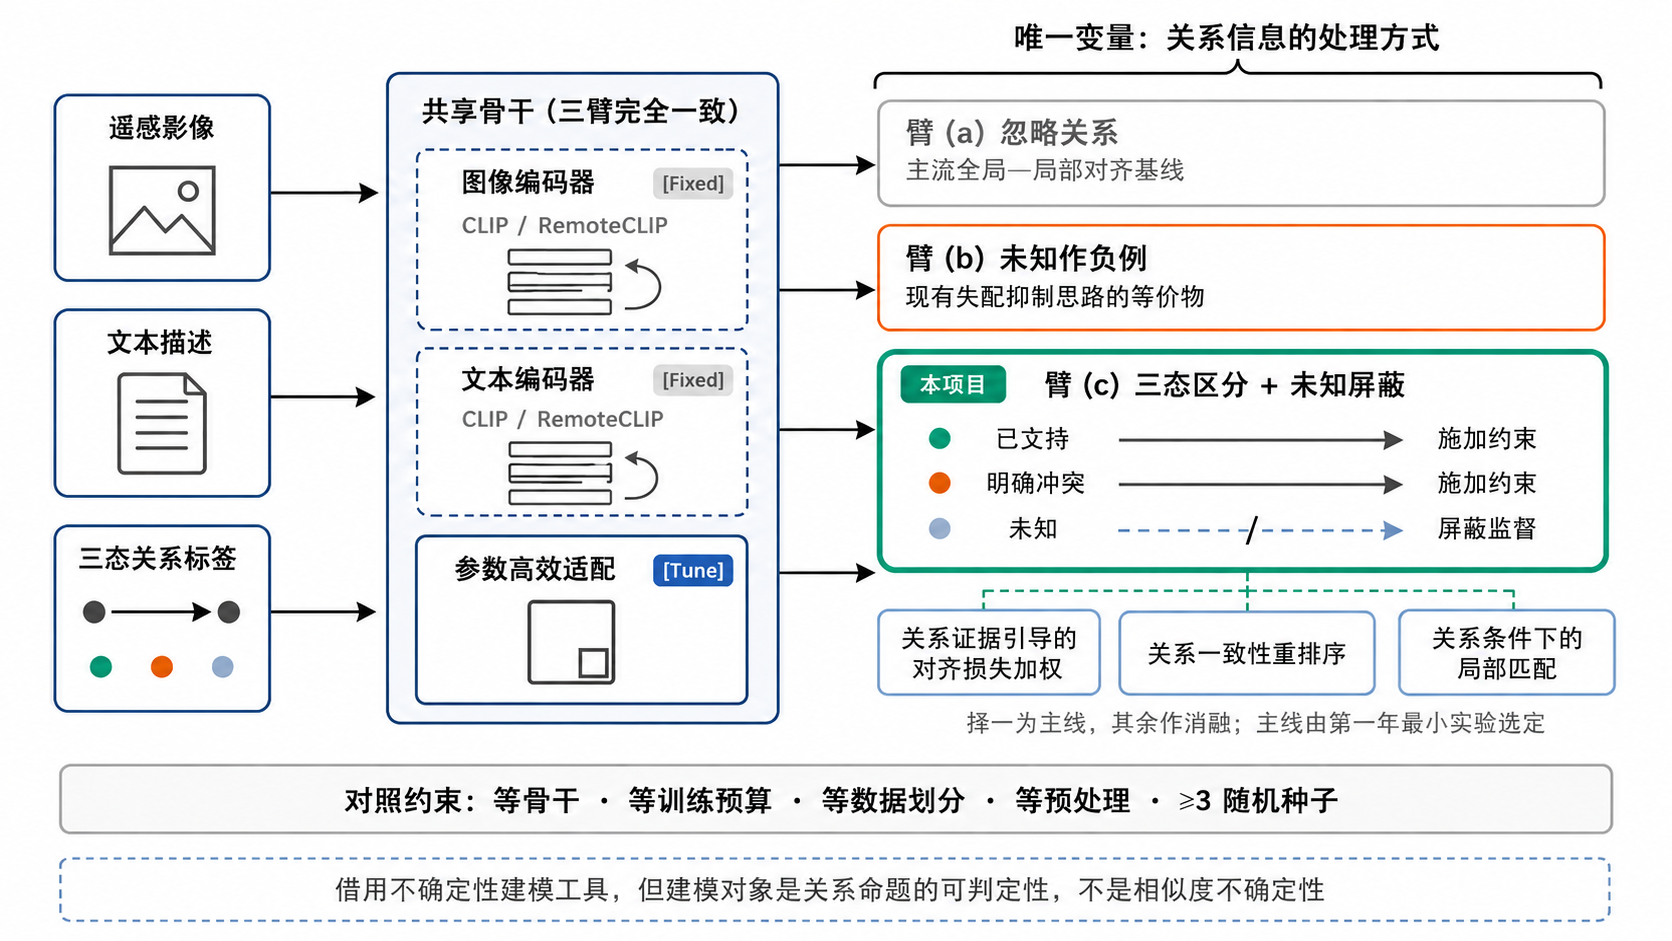
\includegraphics[width=\linewidth]{figures/F06_技术路线二-v2.png}
    \caption{技术路线二：三臂对照的关系约束匹配。三臂保持骨干、训练预算与数据设置一致，仅改变关系信息的处理方式。}
    \label{fig:route-two}
\end{figure}


以已有视觉语言编码器\cite{radford2021clip,liu2024remoteclip}为起点，采用参数高效适配\cite{yuan2023peft,zhou2022cocoop}控制训练规模，研究关系证据参与匹配的方式。本内容的组织方式是\textbf{受控对照}而非模块堆叠，设置三个处理臂：

\begin{enumerate}
    \item \itemtitlefont{臂 (a)：}完全忽略关系信息，对应主流全局--局部对齐基线；
    \item \itemtitlefont{臂 (b)：}把未知关系按负例处理，对应现有失配抑制思路的等价物；
    \item \itemtitlefont{臂 (c)：}区分三态，仅对"已支持"与"明确冲突"施加约束，对"未知"屏蔽监督——本项目主张的处理方式。
\end{enumerate}

臂 (c) 的具体实现有三条候选路线：关系证据引导的对齐损失加权、关系一致性重排序、关系条件下的局部匹配。三者\textbf{择一作为主线}，其余作为消融项，主线由第一年最小实验结果选定。之所以不并列承诺三条路线，是因为本内容要检验的是"三态区分是否有用"，而不是"哪个网络结构更强"；同时纳入过多变量会使结论无法归因。

关系证据的置信度处理可以借用不确定性与证据建模的技术工具\cite{chun2021pcme,han2021tmc,li2023pau,qin2022decl}，但需要明确区分：已有工作建模的是相似度或表示的不确定性，本项目建模的是\textbf{关系命题能否被判定}这一状态。二者在技术实现上可以共享手段，在问题定义上不能混同。

本内容形成的交付物为：核心方法、训练与推理代码、三臂对照与消融结果。

\subsubsubsection{内容三：标准检索与关系挑战的联合验证}

本内容回答"改进如何被归因到关系建模本身"。 联合验证与可归因性控制流程见图~\ref{fig:route-three}。

% F7: F07_技术路线三.png
\begin{figure}[!htbp]
    \centering
    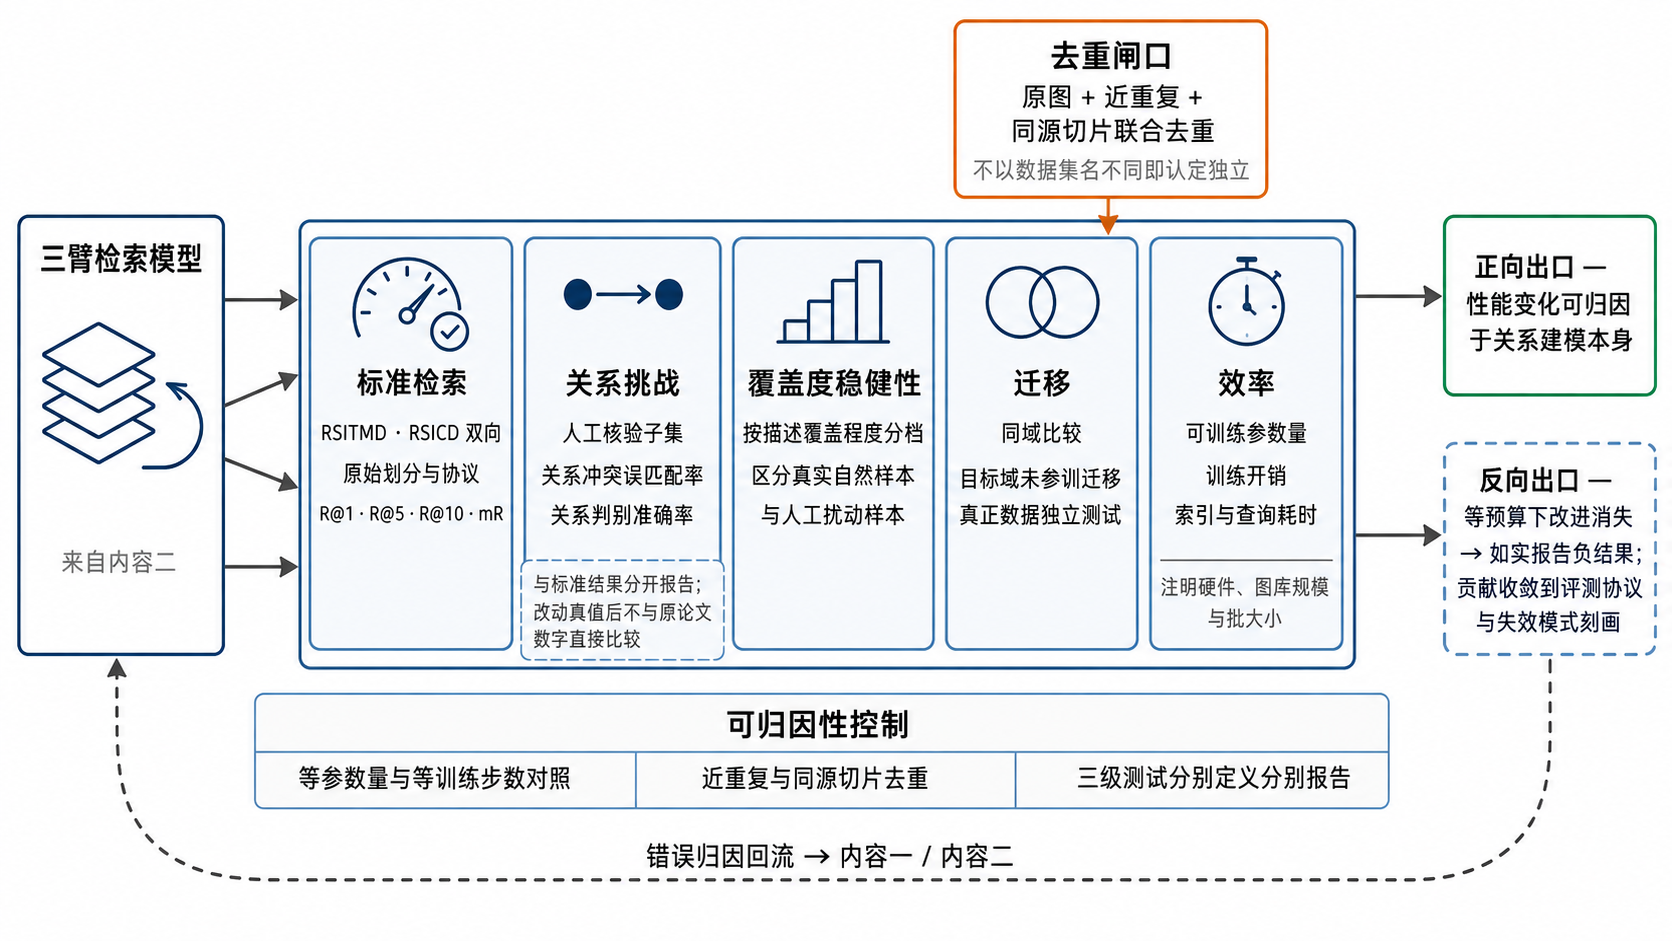
\includegraphics[width=\linewidth]{figures/F07_技术路线三.png}
    \caption{技术路线三：标准检索与关系挑战的联合验证。五维评测分别报告，并以去重和等预算对照检验改进来源。}
    \label{fig:route-three}
\end{figure}


\textbf{标准检索}在 RSITMD\cite{yuan2022amfmn} 与 RSICD\cite{lu2018rsicd} 上进行双向检索，严格沿用原始划分与协议，报告 R@1/R@5/R@10 与六项均值 mR。\textbf{关系挑战评测}在人工核验子集上进行，报告关系冲突误匹配率与关系判别准确率，与标准结果分开呈现——改动标准真值后再与原论文数字直接比较是无效比较。\textbf{覆盖度稳健性评测}按描述覆盖程度分档报告性能变化，并区分真实自然样本与人工扰动样本的结果。

\textbf{可归因性控制}是本内容的重点。包括三项措施：等参数量与等训练步数对照，用于排除容量与预算解释；跨数据集迁移前对原图、近重复影像与同源切片联合去重，不以数据集名称不同就认定相互独立；同域比较、目标域未参与训练的迁移测试、真正数据独立的测试三者分别定义并分别报告。这一要求有直接的现实依据：已有代表性遥感视觉语言模型在训练中使用了与检索基准相关的数据\cite{liu2024remoteclip}，若不加区分地报告，容易把数据重叠带来的收益误读为泛化能力。此外还需报告\textbf{效率指标}：可训练参数量、训练开销、索引与查询耗时，并注明硬件、图库规模与批大小。

本内容形成的交付物为：评测协议、分层结果报告、轻量检索演示与复现材料。

\subsubsubsection{三项内容的独立价值与相互关系}

三项内容在执行上有先后依赖，但各自具备可独立成立的学术价值，不是同一件工作的三个步骤。

内容一产出的实体关系词表、三态判定规范与经人工核验的关系挑战子集，是\textbf{可独立发布的领域资源}：任何研究关系敏感检索、组合泛化或空间语义理解的工作都可直接使用，其价值不依赖于本项目内容二的方法是否成功。内容三产出的分层评测协议同样具有独立性——近重复去重、同域与迁移分别报告、等预算对照这套要求，可用于检验该方向\textbf{其它方法}的结论可归因性，是对领域评测规范的贡献。内容二则是在前两者支撑下对核心假说的直接检验。

正因如此，即使内容二的方法未取得预期效果，内容一与内容三的产出仍然成立并可交付。三者之间还存在一条反馈回路：内容三暴露的失效模式每年回流修订内容一的关系规范与内容二的约束方式，使三项内容构成闭环而非流水线。

\subsubsection{拟解决的关键科学问题}

本项目拟解决的关键科学问题是：\textbf{在遥感图文数据中文本描述对影像内容的覆盖天然不完备的条件下，如何在跨模态匹配中区分"描述未覆盖"与"实际关系冲突"，使有证据的地理实体关系参与约束、而不可判定的关系不被当作监督信号？}

这一问题之所以是科学问题而非工程问题，在于它触及监督信号的合法性来源：对比学习框架默认"未配对即为负例"，而遥感图文数据的结构性不完备使这一默认在相当比例的样本上不成立。回答它需要同时给出状态的可判定表示、状态参与学习的方式，以及使结论可归因的验证设计——这正是三项研究内容的分工。

\subsubsection{研究方法}

本项目采用"数据审计驱动、受控对照检验、分层评测归因"的方法路径。数据审计与标注环节采用分层抽样并先行登记抽样规则，三态判定采用双人独立标注加第三人仲裁，一致性不足的关系类型直接从词表中剔除。模型与训练环节以公开视觉语言编码器为骨干、以参数高效适配控制可训练参数规模，使多种子重复实验在现有算力下可行；三臂对照严格对齐骨干、训练预算、数据划分与预处理，唯一变量是关系信息的处理方式。统计上，关键训练实验至少 3 个随机种子，报告均值、标准差与置信区间，关键对比进行显著性检验。本项目不预设任何提升幅度指标——在完成基线复现之前，任何量化承诺都缺乏依据。

\subsubsection{技术路线}

技术路线为"数据 $\rightarrow$ 关系证据 $\rightarrow$ 匹配方法 $\rightarrow$ 分层验证"的总分结构，并设置一条回流路径。

公开遥感图文数据（RSITMD、RSICD，许可满足时补充少量 SkyScript\cite{wang2024skyscript}）先经数据审计与去重，进入内容一，产出三态关系标签；标签与视觉语言编码器一同进入内容二，通过三臂对照训练得到检索模型；模型在内容三中接受标准检索、关系挑战、覆盖度稳健性、迁移与效率五个维度的分层评测。评测得到的错误归因结果\textbf{每年至少回流一次}：向内容一反馈以修订关系词表与判定规范，向内容二反馈以调整约束方式。

这条回流路径是技术路线的关键设计。关系词表与判定规范不可能一次定稿，只有让评测暴露的失效模式反过来修正表示层，三项内容才构成闭环而非流水线。

\subsubsection{关键技术}

\begin{enumerate}
    \item \itemtitlefont{三态关系证据的判定与表示：}在仅有图像级描述、缺少实体框与拓扑真值的条件下，定义可操作、可复核的三态判据，并处理坐标系依赖与几何增强的标签同步问题。这是本项目最核心也最容易被低估的技术难点。
    \item \itemtitlefont{未知态屏蔽的监督构造：}在对比学习目标中实现"对未知关系不施加监督"，同时避免因屏蔽过多而削弱训练信号；需要在屏蔽比例与训练稳定性之间找到可用区间。
    \item \itemtitlefont{弱标注与人工核验的协同使用：}训练端容忍弱标注噪声、评测端坚持人工核验，二者的边界必须在流程上硬性隔离，防止弱标注污染测试集。
    \item \itemtitlefont{近重复去重与分层评测实施：}对原图、近重复影像与同源切片进行有效识别，并保证同一影像的全部描述落在同一数据划分内。
\end{enumerate}

\subsubsection{可行性分析}

\textbf{理论可行性}：本项目的问题定义建立在已被文献确认的事实之上——遥感图文数据一图多描述、描述覆盖不同地物\cite{lu2018rsicd,yuan2022amfmn}，且现有失配处理方法确实不区分失配成因\cite{pmpguard2026,hu2023rcl,han2023msc}。所需的技术组件（视觉语言编码器、参数高效适配、不确定性建模）均有成熟工作可循\cite{radford2021clip,liu2024remoteclip,yuan2023peft,chun2021pcme,li2023pau}。

\textbf{技术可行性}：三项内容均不依赖尚不存在的技术。内容一是标注规范与数据工程；内容二在成熟编码器上做受控改动，训练规模由参数高效适配控制；内容三是评测协议设计与实施。方法路线刻意避开了从零训练大模型这类高风险高成本路径。

\textbf{数据可行性}：RSITMD 与 RSICD 的公开获取入口已经核验，作者仓库提供影像、标注与解析程序；数据的实际获取与逐样本验证安排在第一年完成，其当前状态详见第（三）部分的前期基础边界说明。

\textbf{条件可行性}：申请人在遥感影像空间结构理解与跨模态检索两个方向的积累恰好构成本项目所需的能力组合，并具备相应的算力与工程基础，详见第（三）部分研究基础与工作条件。

\textbf{风险可控性}：本项目为三条假说均预设了证伪条件与降级路径（详见第（三）部分研究风险与应对措施）。特别地，若第一年的错误归因表明"描述不完备"并非主要误差来源，本项目将据此调整内容一的定位乃至研究题目，而不会通过反向挑选样本维持既定结论。把退出路径写在方案里，本身就是可行性的一部分。
